\section{Background}
\subsection{Multi-Layer Perceptron}
\begin{frame}[c]{Multi-Layer Perceptron}
    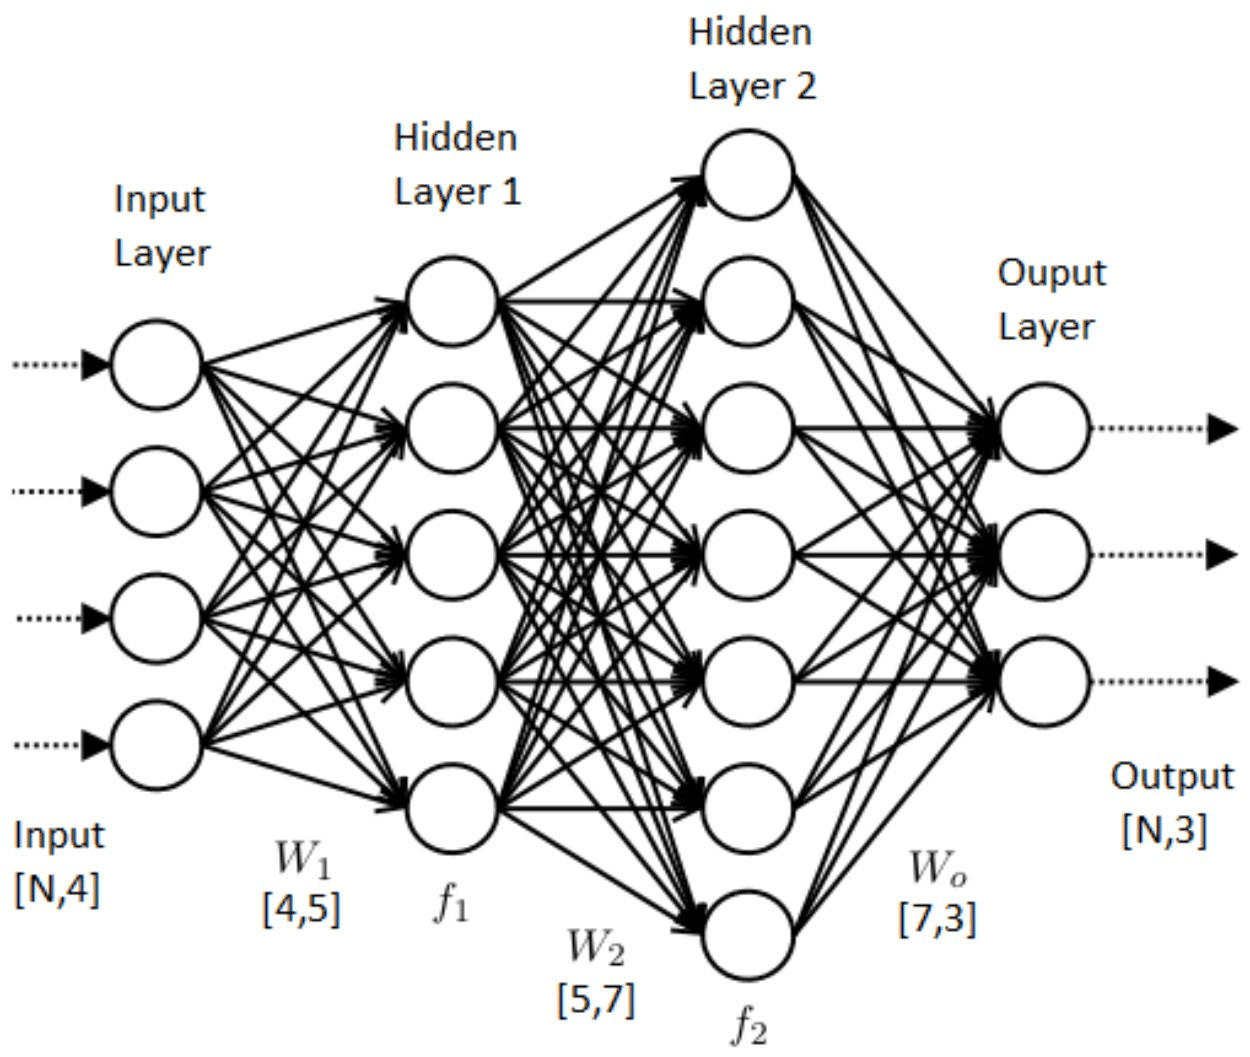
\includegraphics[height=0.85\textheight]{dense_1} \\
    \normalsize
    Image Source: Public Domain
    \pnote{
    Classic Dense FF \\
    has some arbitrary nonlinear activation function
    }
\end{frame}

\subsection{Activation Functions}
\begin{frame}[c]{Common Activation Functions}
    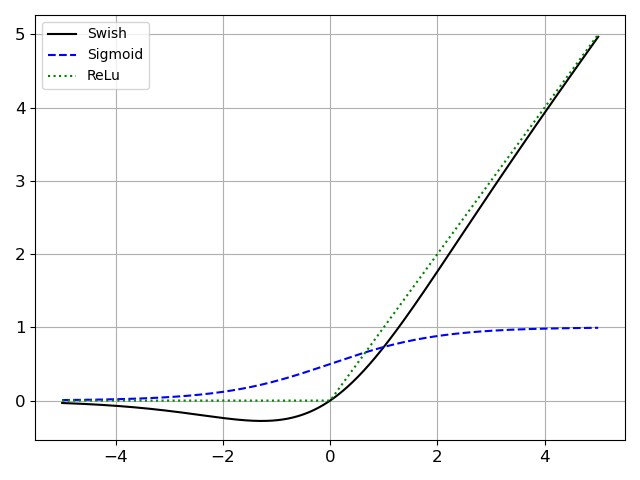
\includegraphics[height=0.75\textheight]{sigmoid_swish_relu} \\
    $swish(x) := x * sigmoid(x)$ \\
    Image Source: \cite{chen_deep_2021} \hspace{1cm}
    SwiGLU introduced by \cite{shazeer_glu_2020}
\end{frame}

\subsection{Dropout}
\begin{frame}[c]{Dropout I}
    \large
    \textbf{Problem: } neural network training results in highly specialized feature adaptations \\
    "Complex co-adaptations can be trained to work well on a training set, but on novel test data they are far more likely to fail than multiple simpler co-adaptations that achieve the same thing." \cite{srivastava_dropout_2014}
\end{frame}

\begin{frame}[c]{Dropout II}
    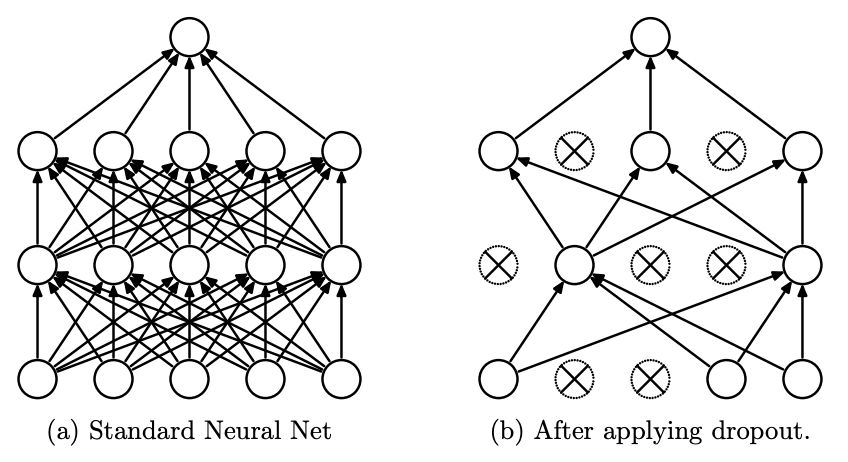
\includegraphics[width=\textwidth]{dropout} \\
    Image Source: \cite{srivastava_dropout_2014}
    \pnote{
        Dropout arbitrarily removes neurons during training \\
        => no reliance on individual features \\
        \\
        Effectively results in an ensamble of different \\
        networks, averaging the output during testing. \\
        Powerful method for regularization
    }
\end{frame}


\subsection{Residual Connections}
\begin{frame}[c]{Residual Connections}
    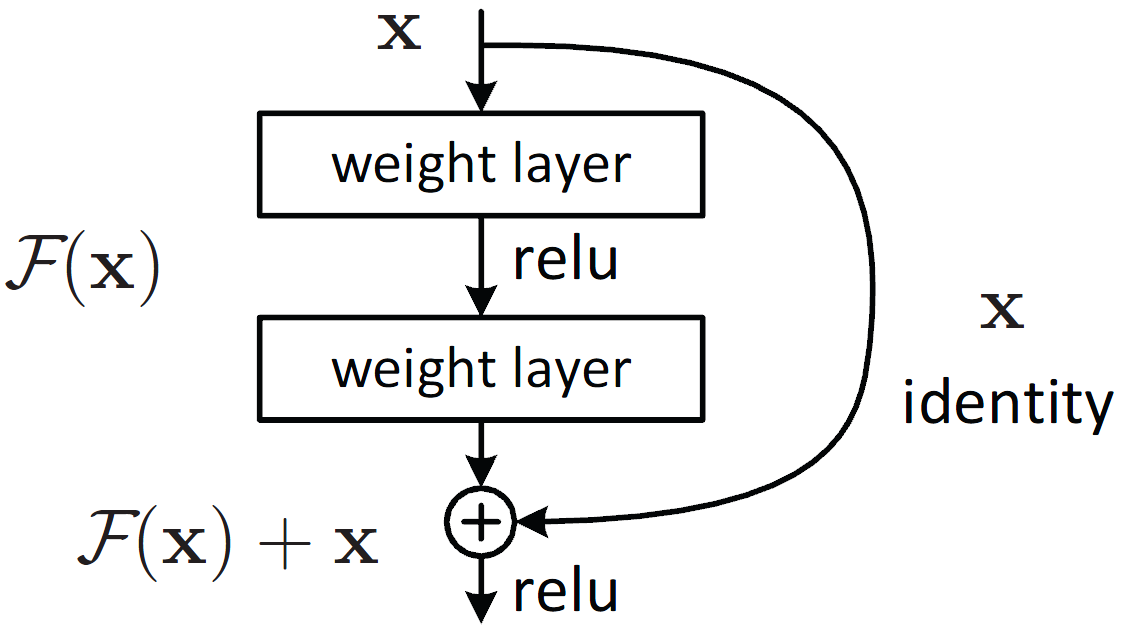
\includegraphics[width=0.8\textwidth]{resnet} \\
    Image Source: \cite{he_deep_2016}
\end{frame}

\begin{frame}[c]{Regularized Residual Connections}
    Self-Regulated Network \cite{xu_regnet_2021}
\end{frame}
